\documentclass[a4paper, 12pt]{article}

\usepackage[top=2cm, bottom=2cm, left=2.5cm, right=2.5cm]{geometry}
\usepackage[utf8]{inputenc}
\usepackage{amsmath, amsfonts, amssymb}
\usepackage{graphicx} % inserir figuras - \includegraphics[scale=•]{•}
\usepackage{float} % ignorar regras de tipografia e inserir figura aonde queremos.
\usepackage[brazil]{babel} % Trocar Figure para Figura.
\usepackage{indentfirst}
\pagestyle{empty}


\begin{document}
\begin{figure}[H]
	
\includegraphics[scale=0.9]{UnB_CiC_Logo.jpg}
\end{figure}
\noindent\rule{\textwidth}{0.4pt}
\begin{center}
	\textbf{{\Large Introdução à Ciência da Computação - 113913}} \newline \newline
	\textbf{{\large Prova 2} \\
	\vspace{9pt}
	{\large Questão A}} \\
	\noindent\rule{\textwidth}{0.4pt}
	\newline
\end{center}

\textbf{{\large Observações:}}
\begin{itemize}
	\item As provas também serão corrigidas por um \textbf{corretor automático}, portanto é necessário que as entradas e saídas do seu programa estejam conforme o padrão especificado em cada questão (exemplo de entrada e saída). Por exemplo, não use mensagens escritas durante o desenvolvimento do seu código como “Informe a primeira entrada”. Estas mensagens não são tratadas pelo corretor, portanto a correção irá resultar em resposta errada, mesmo que seu código esteja correto.
	\item Serão testadas várias entradas além das que foram dadas como exemplo, assim como as listas.
	\item Assim como as listas, as provas devem ser feitas na versão Python 3 ou superior.
	\item \textbf{Questão A valerá 40\% da nota da Prova 2 e a Questão B valerá 60\% da nota da Prova 2}.
	\item Leia com atenção e faça \textbf{exatamente} o que está sendo pedido.
\end{itemize}
\newpage % Questão A 
\begin{center}
\textbf{{\Large Questão A - Brasil}}
\end{center}
\vspace{5pt}
O Brasil é um país de muitas riquezas, mas com muitos problemas. Entre
eles, um dos mais citados nos últimos anos é a corrupção estatal. Sabendo disso, o Ministério da Transparência (antiga Controladoria Geral da
União), criou um sistema de Inteligência Artificial que consegue medir a
probabilidade de um servidor público de se envolver em casos de corrupção,
analisando registros públicos das suas atividades. \newline \newline
Porém, o Ministério da Transparência chegou a um impasse e precisa da
ajuda de um programador Python. Sabendo dos nobres motivos desse
Ministério, você se prontificou para ajudar. Seu trabalho é criar um rankeador para os dados que saem dessa IA. Por sorte, você encontrou o seguinte bilhete em cima da sua mesa:
\begin{figure}[H]
	\centering
	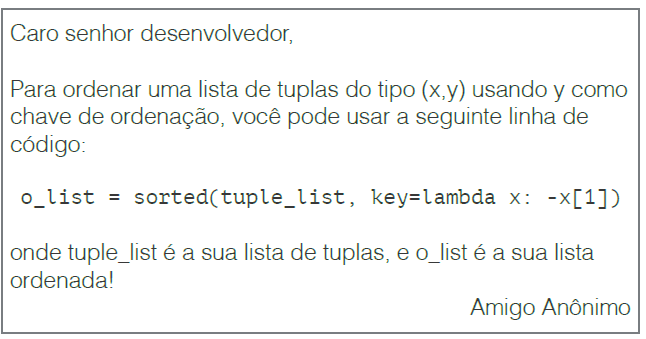
\includegraphics[scale=0.6]{bilhete.png}
\end{figure}
Você pode ajudar? \newline \newline
\textbf{{\large Entrada}} \newline
A primeira linha da entrada consiste de um inteiro \textbf{N}, o número de
funcionários públicos do caso de uso. \newline
As próximas \textbf{N} linhas contêm, cada uma, uma string \textbf{S}, o primeiro nome do
servidor público, e um inteiro \textbf{R}, de 0 a 100, a probabilidade do servidor \textbf{S}
estar envolvido em casos de corrupção.
\newline \newline
\textbf{{\large Saída}} \newline
Seu programa deve imprimir na tela o nome de todos os servidores que têm
\textbf{R} maior que 80, do maior para o menor, em ordem, separados por quebras
de linha. Caso não haja ninguém, imprima ``Ninguém!''.
\newline
\begin{table}[H]
\centering
\begin{tabular}{|l|l|}
\hline
\textbf{Exemplo de Entrada}                                                                       & \textbf{Exemplo de Saída}                                                 \\ \hline
\begin{tabular}[c]{@{}l@{}}4\\ SrCorrupto 99\\ Bezerrinho 87\\ Anjo 10\\ Roberto 100\end{tabular} & \begin{tabular}[c]{@{}l@{}}Roberto\\ SrCorrupto\\ Bezerrinho\end{tabular} \\ \hline
\begin{tabular}[c]{@{}l@{}}3\\ Deboas 10\\ Maisdeboasainda 20\\ Infinitodeboas 30\end{tabular}    & Ninguém!                                                                  \\ \hline
\end{tabular}
\end{table}
\flushright
\textbf{\Large Boa Prova!}
\end{document}